\item \textbf{Find the fourth Taylor polynomial $P_4(x)$ for the function $f (x) = xe^{x^2}$ about $x_0 = 0$.}\\
Como se sabe que
\begin{equation*}
    e^x= \sum_{i=0}^n \frac{x^i}{i!}
\end{equation*}
entonces
\begin{align*}
    f(x) & =xe^{x^2}                                       \\
         & =x \left(\sum_{i=0}^n \frac{(x^2)^i}{i!}\right) \\
         & =  \sum_{i=0}^n x\left(\frac{x^{2i}}{i!}\right) \\
         & = \sum_{i=0}^n \frac{x^{2i+1}}{i!}
\end{align*}
por lo tanto, la función a implementar es:
\begin{equation*}
    f(x)= \sum_{i=0}^n \frac{x^{2i+1}}{i!}
\end{equation*}
\begin{enumerate}
    \item \textbf{Find an upper bound for $|f (x)-P_4 (x)|$, for $0 \leq x \leq 0.4$, ie find an upper bound of $|R_4 (x)|$ for $0 \leq x \leq 0.4$}\\
          Los límites superiores que se encontraron para $|f (x)-P_4 (x)|$ fue 0.000000 y 0.000011 para $|R_4 (x)|$ .
    \item \textbf{Approximate $\int_0^{0.4} f(x)dx$ using $\int_0^{0.4} P_4(x)dx$}\\
          El resultado de la integral usando el polinomio $P_4(x)$ es de 0.086784.
\end{enumerate}
Los resultados anteriores pueden ser verificados en el script contenido en la carpeta \textcolor{citecolor}{Problema\_1}, los valores del salida del programa son los que se muestran en la figura \ref{fig:problema1ss}.
\begin{figure}[H]
    \centering
    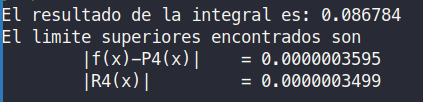
\includegraphics[width=8cm]{Graphics/problema1_ss.png}
    \caption{Captura de pantalla de los valores de salida del programa.}
    \label{fig:problema1ss}
\end{figure}